\subsection{Selection Sort}

Là một thuật toán sắp xếp đơn giản dựa trên việc tìm kiếm 
và đặt phần tử nhỏ nhất (hoặc lớn nhất) vào đúng vị trí 
của nó trong danh sách. Thuật toán này được gọi là "Selection" 
vì mỗi lần lặp, nó chọn phần tử phù hợp để đặt vào vị trí 
chính xác. Đây là một thuật toán không ổn định (unstable) 
vì nếu các phần tử có giá trị bằng nhau, thứ tự ban đầu có thể 
bị thay đổi do hoán vị.

\subsubsection{Ý tưởng}

\begin{enumerate}
    \item Chia danh sách thành hai phần:
    \begin{itemize}[label=$\circ$]
        \item Phần đã sắp xếp (ban đầu trống).
        \item Phần chưa sắp xếp (ban đầu chứa toàn bộ danh sách).
    \end{itemize}
    \item Lặp qua danh sách:
    \begin{itemize}[label=$\circ$]
        \item Tìm phần tử nhỏ nhất trong phần chưa sắp xếp.
        \item Hoán đổi phần tử nhỏ nhất này với phần tử đầu tiên 
        của phần chưa sắp xếp.
    \end{itemize}
    \item Sau mỗi lần hoán đổi, mở rộng phần đã sắp xếp thêm 
    một phần tử.
    \item Tiếp tục cho đến khi toàn bộ danh sách được sắp xếp.
\end{enumerate}

\subsubsection{Mã giả}

\begin{algorithm}[H]
\caption{Selection Sort}
\SetKwFunction{SelectionSort}{SelectionSort}
\SetKwProg{Fn}{Function}{:}{}
\Fn{\SelectionSort{a\KwSty{[]}, n}}{
    \For{$i \gets 0$ \KwTo $n-2$}{
        // Bước 1: Giả định phần tử nhỏ nhất là a[i] \\
        $minIndex \gets i$ \\
        // Bước 2: Tìm phần tử nhỏ nhất trong phần chưa sắp xếp \\
        \For{$j \gets i+1$ \KwTo $n-1$}{
            \If{$a[j] < a[minIndex]$}{
                $minIndex \gets j$ \\
            }
        }
        // Bước 3: Hoán đổi phần tử nhỏ nhất với a[i] \\
        \If{$minIndex \neq i$}{
            swap($a[i]$, $a[minIndex]$) \\
        }
    }
}
\textbf{end function}
\end{algorithm}

\subsubsection{Ví dụ}

Giả sử ta có mảng ban đầu với $n=5$ như sau:
\begin{center}
    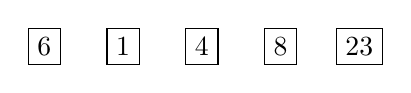
\begin{tikzpicture}
        \node[draw, fill=white] at (9, 0) {6};
        \node[draw, fill=white] at (10, 0) {1};
        \node[draw, fill=white] at (11, 0) {4};
        \node[draw, fill=white] at (12, 0) {8};
        \node[draw, fill=white] at (13, 0) {23};
    \end{tikzpicture}
\end{center}

\textbf{Bước 1:} Bắt đầu từ phần tử đầu tiên tại vị trí $i=0$, 
tìm phần tử nhỏ nhất trong phần mảng chưa sắp xếp $(1)$ và 
hoán vị với phần tử hiện tại $(6)$.

\begin{center}
    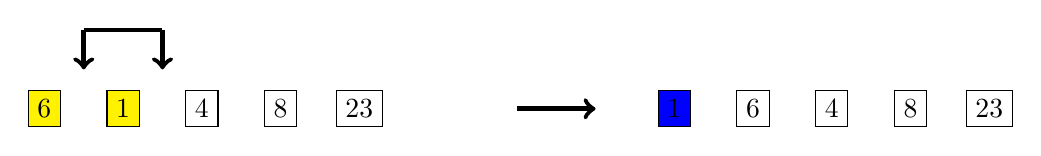
\begin{tikzpicture}
        \node[draw, fill=yellow] at (1, -3.5) {6};
        \node[draw, fill=yellow] at (2, -3.5) {1};
        \node[draw, fill=white] at (3, -3.5) {4};
        \node[draw, fill=white] at (4, -3.5) {8};
        \node[draw, fill=white] at (5, -3.5) {23};
        \draw[<-, line width=0.6mm, shorten <=0pt] (2.5, -3) -- (2.5, -2.5);
        \draw[line width=0.6mm] (2.5, -2.5) -- (1.5, -2.5);
        \draw[->, line width=0.6mm, shorten >=0pt] (1.5, -2.5) -- (1.5, -3);
        
        \draw[->, line width=0.6mm] (7, -3.5) -- (8, -3.5);
        
        \node[draw, fill=blue] at (9, -3.5) {1};
        \node[draw, fill=white] at (10, -3.5) {6};
        \node[draw, fill=white] at (11, -3.5) {4};
        \node[draw, fill=white] at (12, -3.5) {8};
        \node[draw, fill=white] at (13, -3.5) {23};
    \end{tikzpicture}
\end{center}
	
\textbf{Bước 2:} Chuyển đến phần tử tiếp theo tại vị trí $i=1$, 
tìm phần tử nhỏ nhất trong phần mảng chưa sắp xếp $(4)$ và 
hoán vị với phần tử hiện tại $(6)$.

\begin{center}
    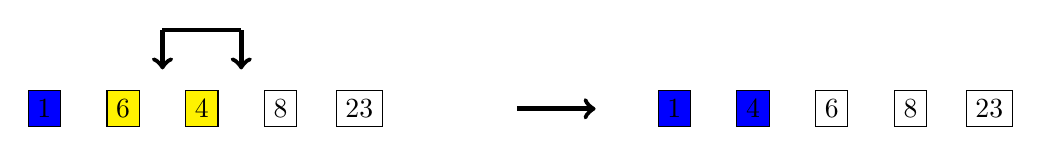
\begin{tikzpicture}
        \node[draw, fill=blue] at (1, -7) {1};
        \node[draw, fill=yellow] at (2, -7) {6};
        \node[draw, fill=yellow] at (3, -7) {4};
        \node[draw, fill=white] at (4, -7) {8};
        \node[draw, fill=white] at (5, -7) {23};
        \draw[<-, line width=0.6mm, shorten <=0pt] (3.5, -6.5) -- (3.5, -6);
        \draw[line width=0.6mm] (3.5, -6) -- (2.5, -6);
        \draw[->, line width=0.6mm, shorten >=0pt] (2.5, -6) -- (2.5, -6.5);
        
        \draw[->, line width=0.6mm] (7, -7) -- (8, -7);
        
        \node[draw, fill=blue] at (9, -7) {1};
        \node[draw, fill=blue] at (10, -7) {4};
        \node[draw, fill=white] at (11, -7) {6};
        \node[draw, fill=white] at (12, -7) {8};
        \node[draw, fill=white] at (13, -7) {23};
    \end{tikzpicture}
\end{center}

Do phần còn lại của mảng đã theo thứ tự nên các bước tiếp theo sẽ 
không có sự thay đổi và cuối cùng ta được mảng đã sắp xếp:

\begin{center}
    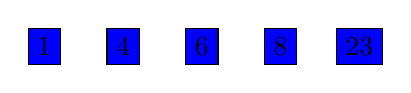
\begin{tikzpicture}
        \node[draw, fill=blue] at (0, 0) {1};
        \node[draw, fill=blue] at (1, 0) {4};
        \node[draw, fill=blue] at (2, 0) {6};
        \node[draw, fill=blue] at (3, 0) {8};
        \node[draw, fill=blue] at (4, 0) {23};
    \end{tikzpicture}
\end{center}

\subsubsection{Độ phức tạp thuật toán}

\begin{itemize}
    \item Độ phức tạp thời gian
    \begin{itemize}[label=$\circ$]
        \item Trường hợp tốt nhất: $O\left(n^2\right)$.
        \item Trường hợp xấu nhất: $O\left(n^2\right)$.
        \item Trung bình: $O\left(n^2\right)$ vì thuật toán sử dụng 
        hai vòng lặp lồng nhau để tìm phần tử nhỏ nhất.
    \end{itemize}
    \item Độ phức tạp không gian: $O\left(1\right)$ vì không sử dụng 
    bộ nhớ bổ sung ngoài danh sách ban đầu.
\end{itemize}